\documentclass{article}
\usepackage{graphicx}
\usepackage{amsmath}
\usepackage{amsfonts}
\author{Guangyao Zhou}
\title{Show, Attend and Distill: Knowledge Distillation via Attention-based Feature Matching}
\begin{document}	
	\maketitle
	\begin{figure*}[t]
		\centering
		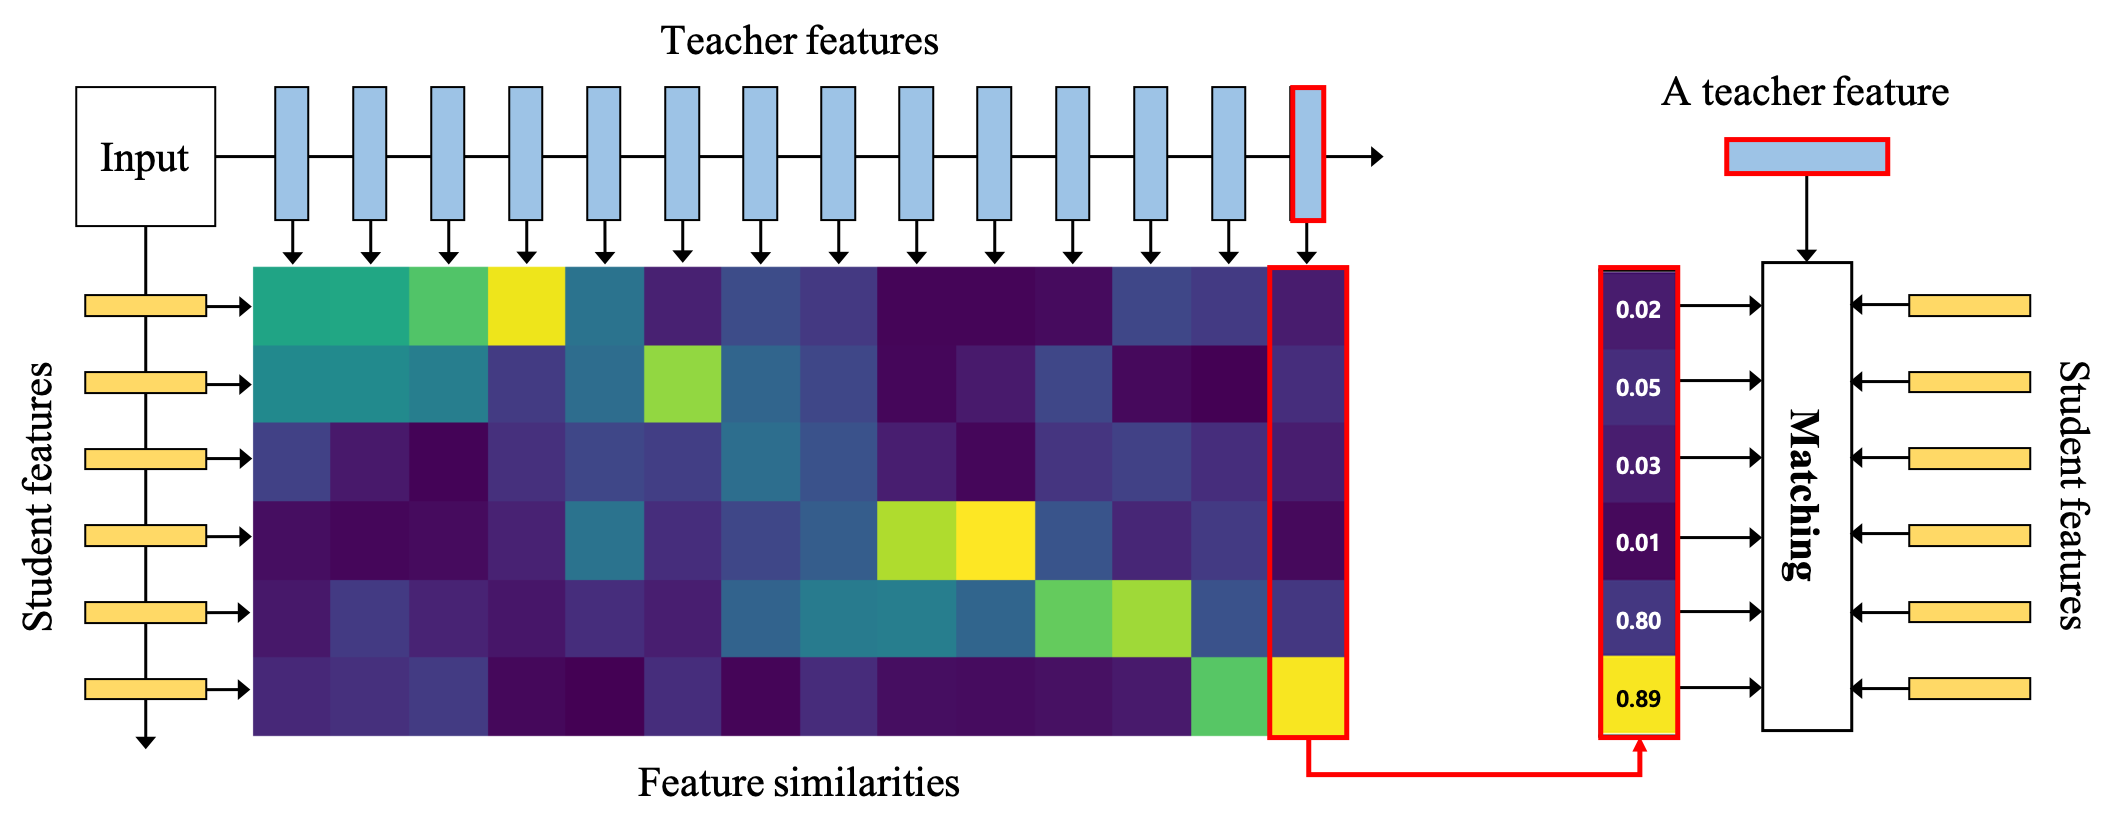
\includegraphics[width=\columnwidth]{figure/Figure1_sr.png}
		\caption{Overview of AFD. An attention-based model determines similarities between the teacher and student features. Knowledge from each teacher feature is transferred to the student with the identified similarities.}
		\label{fig:overview}
	\end{figure*}
	\section{Abstract}
	\subsection{Motivation}
	Manual link selection does not consider the similarity between the teacher and student features, so there is a risk of forcing an incorrect intermediate process to the student. Furthermore, he link selection has a limitation on fully utilizing the whole knowledge of the teacher by choosing a few of all possible links.
	\subsection{Preworks}
	Most studies manually tie intermediate features of the teacher and student, and transfer knowledge through predefined links.
	\subsection{Approach}
	The authors proposed method utilizes an attention-based meta-network that learns relative similarities between features.
	\subsection{Contribution}
	The authors proposed method determines competent links more efficiently
	\section{Related Preworks}
	\subsection{Learning to Transfer (L2T)}
	\subsubsection{L2T Approach}
	To compensate for the limitation, Jang \textit{et al.} [Learning What and Where to Transfer] apply a meta-networks, ``learning to transfer (L2T)'', automatically determining the links.
	In more details, the meta-network consists of individual gates for all possible links, and each gate determines whether distillation through the link contributes to decreasing the classification loss of the student.
	\subsubsection{1st Con}
	\textit{The connections ae not aware that ther're affecting simultaneously}\\
	The individual gates are not aware of each other although the distillation through the gates simultaneously affect the student. 
	\subsubsection{2nd Con}
	\textit{Computational Expensive}\\
	The meta-learning scheme requires expensive inner-loop procedures to learn their meta-networks, thus its application can be limited under practical scenarios.
	%\subsection{Attention-based Feature Distillation (AFD)}
	%\subsubsection{AFD Approach}
	%AFD (Xue \textit{et al.} [Show, attend and tell: Neural image caption generation with visual attention]; Vaswani \textit{et al.} [Attention is all you need])utilizes an attention-based meta-network that identifies similar features between the teacher and student.
	\subsection{Advantages Compare to L2T}
	\begin{itemize}
		\item[i] The authors proposed method considers the granularity of the teacher and student features to identify the importance of their links while L2T only uses information for a single pair in a narrow perspective.
		\item[ii] AFD learns from feature similarities without any inner-loop procedure but L2T learns from the classification loss, which requires expensive Hessian computation.
	\end{itemize}
	\section{Attention-based Feature Distillation}
	\begin{figure*}[t]
		\centering
		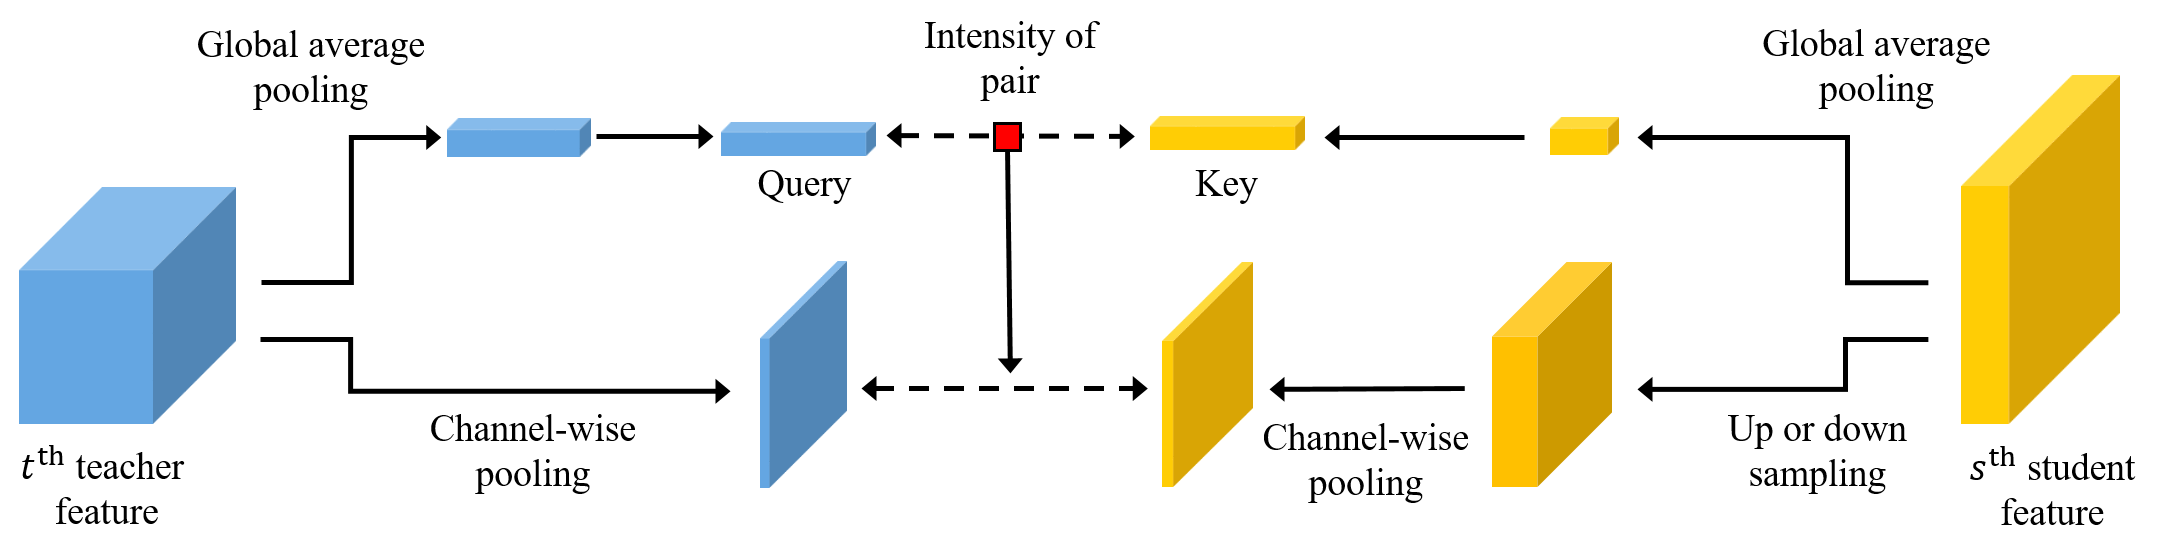
\includegraphics[width=\columnwidth]{figure/Figure2_intensity.png}
		\caption{Overview of the proposed meta-network. The globally pooled features are utilized to estimate the similarities and the channel-wisely averaged features are used to calculate the distance between the features.}
		\label{fig:method}
	\end{figure*}
	Let $\mathbf{h}^{\text{T}}=\{{h}^{\text{T}}_1, ..., {h}^{\text{T}}_T\}$ be a set of the feature candidates from the teacher and $\mathbf{h}^{\text{S}}=\{{h}^{\text{S}}_1, ..., {h}^{\text{S}}_S\}$ be a set of feature candidates from the student where $T$ and $S$ indicate the numbers of the candidates from the teacher and student, respectively.\\
	Specifically, each teacher feature generates a query, $\mathbf{q}_t$, and each student feature identifies a key, $\mathbf{k}_{s}$. \\
	\begin{equation}
		\begin{aligned}
			& \mathbf{q}_t = f_Q ( W^{\text{Q}}_t \cdot \phi^{HW}({h}^{\text{T}}_t) ), \\
			& \mathbf{k}_{s} = f_K ( W^{\text{K}}_s \cdot \phi^{HW}({h}^{\text{S}}_s) ).
		\end{aligned}
	\end{equation}
	$\phi^{HW}( \cdot )$ indicates a global average pooling. $f_Q$ and $f_K$ are activation function of the query and key. $W^{\text{Q}}_t \in \mathbb{R}^{d \times d^{\text{T}}_t}$ and $W^{\text{K}}_s \in \mathbb{R}^{d \times d^{\text{S}}_s}$ are linear transition parameters for the $t$-th query and the $s$-th key.\\
	\begin{equation}
		\begin{aligned}
			\mathbf{\alpha}_t={}&\text{softmax} ( [(\mathbf{q}_t^\top W_1^ {\text{Q-K}} \mathbf{k}_{t,1} + (\mathbf{p}_t^{\text{T}})^\top \mathbf{p}_{1}^{\text{S}}) / \sqrt{d}, \\
			& \cdots , (\mathbf{q}_t^\top W_S^{\text{Q-K}}\mathbf{k}_{t,S} + (\mathbf{p}_t^{\text{T}})^\top \mathbf{p}_{S}^{\text{S}}) / \sqrt{d} ]).
		\end{aligned}
	\end{equation}
	Here, The authors introduce additional weight parameters; a bilinear weight, $W_t^{\text{Q-K}}\in \mathbb{R}^{d \times d}$, and positional encodings, $\mathbf{p}_{t}^{\text{T}} \in  \mathbb{R}^{d}$ and $\mathbf{p}_{s}^{\text{S}}\in  \mathbb{R}^{d}$. The bilinear weight is applied to generalize the attention value from different source ranks since the query and key are identified from different dimensional features~\cite{bilinear-1,bilinear-2}. The positional encodings are utilized to share common information over different instances~\cite{transformer}. $\mathbf{\alpha}_t$ is the attention vector that capture relation between the $t$-th teacher feature and whole student features. By utilizing $\mathbf{\alpha}_t$, the teacher feature, ${h}^{\text{T}}_t$, enables to transfer its knowledge selectively to student features.\\
	The final distillation term forms as
	\begin{equation}
		\mathcal{L}_{\text{AFD}} = \Sigma_{t}{\Sigma_{s}{ \alpha_{t,s} \left\Vert
				\tilde{\phi}^{C}({h}^{\text{T}}_t) - \tilde{\phi}^{C}(\hat{h}^{\text{S}}_s)
				\right\Vert_2 }},
		\label{eq:sad_loss}
	\end{equation}
	where $\tilde{\phi}^{C}$ indicates a combined function of a channel-wise average pooling layer with L2 normalization, $\mathbf{v}/\left\Vert \mathbf{v} \right\Vert_2$, by following \cite{atts}. In addition, $\hat{h}^{\text{S}}_s$ is up-sampled or down-sampled from $h^{\text{S}}_s$ to match the feature map size to those of the teacher features. \\
	Finally, the regularization term is added to the total loss function as following;
	\begin{equation}
		\mathcal{L}_{\text{Student}} = \mathcal{L}_{\text{cls}} + \beta \mathcal{L}_{\text{AFD}},
	\end{equation}
\end{document}